\documentclass[10pt]{article}
\usepackage[utf8]{inputenc}
\usepackage[T1]{fontenc}
\usepackage{amsmath}
\usepackage{amsfonts}
\usepackage{amssymb}
\usepackage[version=4]{mhchem}
\usepackage{stmaryrd}
\usepackage{graphicx}
\usepackage[export]{adjustbox}
\graphicspath{ {./images/} }
\usepackage{bbold}

\begin{document}
\section*{MATHEMATICS}
\section*{SECTION-A}
\begin{enumerate}
  \setcounter{enumi}{60}
  \item Let \(A=\left(\begin{array}{cc}m & n \\ p & q\end{array}\right), d=|A| \neq 0|A-d(\operatorname{Adj} A)|=0\)\\
. Then\\
(1) \((1+d)^{2}=(m+q)^{2}\)\\
(2) \(1+\mathrm{d}^{2}=(\mathrm{m}+\mathrm{q})^{2}\)\\
(3) \((1+d)^{2}=m^{2}+q^{2}\)\\
(4) \(1+\mathrm{d}^{2}=\mathrm{m}^{2}+\mathrm{q}^{2}\)
\end{enumerate}

\section*{Official Ans. by NTA (1)}
Allen Ans. (1)\\
Sol. \(\quad A=\left[\begin{array}{cc}m & n \\ p & q\end{array}\right], \quad|A-d(\operatorname{adj} A)|=0\)\\
\(\Rightarrow|A-d(\operatorname{adj} A)|=\left|\left[\begin{array}{cc}m & n \\ p & q\end{array}\right]-d\left[\begin{array}{cc}q & -n \\ -p & m\end{array}\right]\right|\)\\
\(=\left|\begin{array}{cc}\mathrm{m}-\mathrm{qd} & \mathrm{n}(1+\mathrm{d}) \\ \mathrm{p}(1+\mathrm{d}) & \mathrm{q}-\mathrm{md}\end{array}\right|=0\)\\
\(\Rightarrow \quad(\mathrm{m}-\mathrm{qd})(\mathrm{q}-\mathrm{md})-\mathrm{np}(1+\mathrm{d})^{2}=0\)\\
\(\Rightarrow \quad \mathrm{mq}-\mathrm{m}^{2} \mathrm{~d}-\mathrm{q}^{2} \mathrm{~d}+\mathrm{mqd}^{2}-\mathrm{np}(1+\mathrm{d})^{2}=0\)\\
\(\Rightarrow \quad(\mathrm{mq}-\mathrm{np})+\mathrm{d}^{2}(\mathrm{mq}-\mathrm{np})-\mathrm{d}\left(\mathrm{m}^{2}+\mathrm{q}^{2}+2 \mathrm{np}\right)=0\)\\
\(\Rightarrow \quad d+d^{3}-d\left((m+q)^{2}-2 d\right)=0\)\\
\(\Rightarrow \quad 1+\mathrm{d}^{2}=(\mathrm{m}+\mathrm{q})^{2}-2 \mathrm{~d}\)\\
\(\Rightarrow \quad(1+\mathrm{d})^{2}=(\mathrm{m}+\mathrm{q})^{2}\)\\
\(\therefore\) Option (1) is correct.\\
62. The line \(l_{1}\) passes through the point \((2,6,2)\) and is perpendicular to the plane \(2 \mathrm{x}+\mathrm{y}-2 \mathrm{z}=10\). Then the shortest distance between the line \(1_{1}\) and the line \(\frac{x+1}{2}=\frac{y+4}{-3}=\frac{z}{2}\) is :\\
(1) 7\\
(2) \(\frac{19}{3}\)\\
(3) \(\frac{19}{3}\)\\
(4) 9

\section*{Official Ans. by NTA (4)}
Allen Ans. (4)

\section*{TEST PAPER WITH SOLUTION}
Sol. Line \(\ell\), is given by\\
\(\mathrm{L}_{1}: \frac{\mathrm{x}-2}{2}=\frac{\mathrm{y}-6}{1}=\frac{\mathrm{z}-2}{-2}\)\\
Given,\\
\(\mathrm{L}_{2}: \frac{\mathrm{x}+1}{2}=\frac{\mathrm{y}+4}{-3}=\frac{\mathrm{z}}{2}\)\\
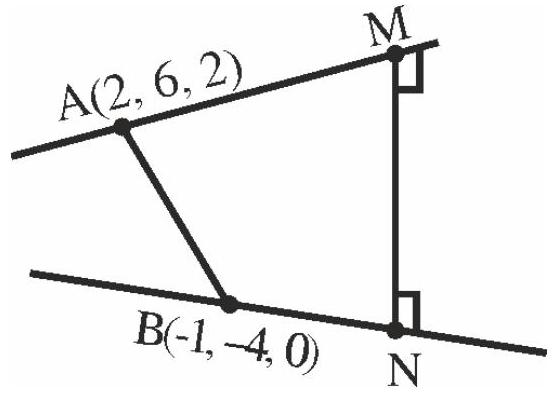
\includegraphics[max width=\textwidth, center]{2025_10_03_96e86532e9cc1b08fca5g-01}

Shortest distance \(=\left|\frac{\overrightarrow{\mathrm{AB}} \cdot \overrightarrow{\mathrm{MN}}}{\mathrm{MN}}\right|\)\\
\(\overrightarrow{\mathrm{AB}}=3 \hat{\mathrm{i}}+10 \hat{\mathrm{j}}+2 \hat{\mathrm{k}}\)\\
\(\overrightarrow{\mathrm{MN}}=\left|\begin{array}{ccc}\hat{i} & \hat{j} & \hat{k} \\ 2 & 1 & -2 \\ 2 & -3 & 2\end{array}\right|=-4 \hat{i}-8 \hat{j}-8 \hat{k}\)\\
\(\mathrm{MN}=\sqrt{16+64+64}=12\)\\
\(\therefore \quad\) Shortest distance \(=\left|\frac{-12-80-16}{12}\right|=9\)\\
\(\therefore\) Option (4) is correct.\\
63. If an unbiased die, marked with \(-2,-1,0,1,2,3\) on its faces, is through five times, then the probability that the product of the outcomes is positive, is :\\
(1) \(\frac{881}{2592}\)\\
(2) \(\frac{521}{2592}\)\\
(3) \(\frac{440}{2592}\)\\
(4) \(\frac{27}{288}\)

Official Ans. by NTA (2)\\
Allen Ans. (2)

Sol. Either all outcomes are positive or any two are negative.

Now, \(p=P(\) positive \()=\frac{3}{6}=\frac{1}{2}\)\\
\(\mathrm{q}=\mathrm{p}(\) negative \()=\frac{2}{6}=\frac{1}{3}\)\\
Required probability\\
\(={ }^{5} \mathrm{C}_{5}\left(\frac{1}{2}\right)^{5}+{ }^{5} \mathrm{C}_{2}\left(\frac{1}{3}\right)^{2}\left(\frac{1}{2}\right)^{3}+{ }^{5} \mathrm{C}_{4}\left(\frac{1}{3}\right)^{4}\left(\frac{1}{2}\right)^{1}\)\\
\(=\frac{521}{2592}\)\\
\(\therefore \quad\) Option (2) is correct.\\
64. Let the system of linear equations\\
\(\mathrm{x}+\mathrm{y}+\mathrm{kz}=2\)\\
\(2 x+3 y-z=1\)\\
\(3 x+4 y+2 z=k\)\\
have infinitely many solutions. Then the system\\
\((\mathrm{k}+1) \mathrm{x}+(2 \mathrm{k}-1) \mathrm{y}=7\)\\
\((2 \mathrm{k}+1) \mathrm{x}+(\mathrm{k}+5) \mathrm{y}=10\) has :\\
(1) infinitely many solutions\\
(2) unique solution satisfying \(x-y=1\)\\
(3) no solution\\
(4) unique solution satisfying \(x+y=1\)

Official Ans. by NTA (4)\\
Allen Ans. (4)\\
Sol. \(\left|\begin{array}{ccc}1 & 1 & \mathrm{k} \\ 2 & 3 & -1 \\ 3 & 4 & 2\end{array}\right|=0\)\\
\(\Rightarrow \quad 1(10)-1(7)+\mathrm{k}(-1)-0\)\\
\(\Rightarrow \quad \mathrm{k}=3\)\\
For \(\mathrm{k}=3,2^{\text {nd }}\) system is\\
\(4 x+5 y=7\)\\
and \(7 x+8 y=10\)

Clearly, they have a unique solution\\
(2) - (1) \(\Rightarrow 3 \mathrm{x}+3 \mathrm{y}=3\)\\
\(\Rightarrow \mathrm{x}+\mathrm{y}=1\)\\
65. If \(\tan 15^{\circ}+\frac{1}{\tan 75^{\circ}}+\frac{1}{\tan 105^{\circ}}+\tan 195^{\circ}=2 \mathrm{a}\), then the value of \(\left(a+\frac{1}{a}\right)\) is :\\
(1) 4\\
(2) \(4-2 \sqrt{3}\)\\
(3) 2\\
(4) \(5-\frac{3}{2} \sqrt{3}\)

Official Ans. by NTA (1)\\
Allen Ans. (1)\\
Sol. Option (1)\\
\(\tan 15^{\circ}=2-\sqrt{3}\)\\
\(\frac{1}{\tan 75^{\circ}}=\cot 75^{\circ}=2-\sqrt{3}\)\\
\(\frac{1}{\tan 105^{\circ}}=\cot \left(105^{\circ}\right)=-\cot 75^{\circ}=\sqrt{3}-2\)\\
\(\tan 195^{\circ}=\tan 15^{\circ}=2-\sqrt{3}\)\\
\(\therefore \quad 2(2-\sqrt{3})=2 a \quad \Rightarrow a=2-\sqrt{3}\)\\
\(\Rightarrow \quad a+\frac{1}{a}=4\)\\
66. Suppose \(\mathrm{f}: \mathrm{R} \rightarrow(0, \infty)\) be a differentiable function such that \(5 f(x+y)=f(x) \cdot f(y), \forall x, y \in R\).

If\\
\(f(3)=320\), then \(\sum_{n=0}^{5} f(n)\) is equal to :\\
(1) 6875\\
(2) 6575\\
(3) 6825\\
(4) 6528

Official Ans. by NTA (3)\\
Allen Ans. (3)\\
Sol. Option (3)

\[
\begin{array}{ll} 
& 5 \mathrm{f}(\mathrm{x}+\mathrm{y})=\mathrm{f}(\mathrm{x}) \cdot \mathrm{f}(\mathrm{y}) \\
& 5 \mathrm{f}(0)=\mathrm{f}(0)^{2} \Rightarrow \mathrm{f}(0)=5 \\
& 5 \mathrm{f}(\mathrm{x}+1)=\mathrm{f}(\mathrm{x}) \cdot \mathrm{f}(1) \\
\Rightarrow & \frac{\mathrm{f}(\mathrm{x}+1)}{\mathrm{f}(\mathrm{x})}=\frac{\mathrm{f}(1)}{5} \\
\Rightarrow & \frac{\mathrm{f}(1)}{\mathrm{f}(0)} \cdot \frac{\mathrm{f}(2)}{\mathrm{f}(1)} \cdot \frac{\mathrm{f}(3)}{\mathrm{f}(2)}=\left(\frac{\mathrm{f}(1)}{5}\right)^{3} \\
\Rightarrow \quad & \frac{320}{5}=\frac{(\mathrm{f}(1))^{3}}{5^{3}} \Rightarrow \mathrm{f}(1)=20 \\
\therefore \quad & 5 \mathrm{f}(\mathrm{x}+1)=20 \cdot \mathrm{f}(\mathrm{x}) \Rightarrow \mathrm{f}(\mathrm{x}+1)=4 \mathrm{f}(\mathrm{x}) \\
& \sum_{\mathrm{n}=0}^{5} \mathrm{f}(\mathrm{n})=5+5.4+5.4^{2}+5.4^{3}+5.4^{4}+5.4^{5} \\
& =\frac{5\left[4^{6}-1\right]}{3}=6825
\end{array}
\]

\begin{enumerate}
  \setcounter{enumi}{66}
  \item If \(\mathrm{a}_{\mathrm{n}}=\frac{-2}{4 \mathrm{n}^{2}-16 \mathrm{n}+15}\), then \(\mathrm{a}_{1}+\mathrm{a}_{2}+\ldots .+\mathrm{a}_{25}\) is equal to:\\
(1) \(\frac{51}{144}\)\\
(2) \(\frac{49}{138}\)\\
(3) \(\frac{50}{141}\)\\
(4) \(\frac{52}{147}\)
\end{enumerate}

Official Ans. by NTA (3)\\
Allen Ans. (3)\\
Sol. Option (3)\\
If \(\mathrm{a}_{\mathrm{n}}=\frac{-2}{4 \mathrm{n}^{2}-16 \mathrm{n}+15}\) then \(\mathrm{a}_{1}+\mathrm{a}_{2}+\ldots \ldots . \mathrm{a}_{25}\)\\
\(\Rightarrow \quad \sum_{n=1}^{25} a_{n}=\sum \frac{-2}{4 n^{2}-16 n+15}\)\\
\(=\sum \frac{-2}{4 n^{2}-6 n-10 n+15}\)\\
\(=\sum \frac{-2}{2 n(2 n-3)-5(2 n-3)}\)\\
\(=\sum \frac{-2}{(2 n-3)(2 n-5)}\)\\
\(=\sum \frac{1}{2 n-3}-\frac{1}{2 n-5}\)\\
\(=\frac{1}{47}-\frac{1}{(-3)}\)\\
\(=\frac{50}{141}\)\\
68. If the coefficient of \(x^{15}\) in the expansion of \(\left(a x^{3}+\frac{1}{b x^{\frac{1}{3}}}\right)^{15}\) is equal to the coefficient of \(x^{-15}\) in the expansion of \(\left(a x^{\frac{1}{3}}-\frac{1}{b x^{3}}\right)^{15}\), where \(a\) and \(b\) are positive real numbers, then for each such ordered pair (a, b) :\\
(1) \(a=b\)\\
(2) \(\mathrm{ab}=1\)\\
(3) \(a=3 b\)\\
(4) \(\mathrm{ab}=3\)

Official Ans. by NTA (2)\\
Allen Ans. (2)

Sol. Option (2)\\
Coefficient Of \(\mathrm{x}^{15}\) in \(\left(\mathrm{ax}^{3}+\frac{1}{\mathrm{bx}^{1 / 3}}\right)^{15}\)\\
\(\mathrm{T}_{\mathrm{r}+1}={ }^{15} \mathrm{C}_{\mathrm{r}}\left(\mathrm{ax}^{3}\right)^{15-\mathrm{r}}\left(\frac{1}{\mathrm{bx}^{1 / 3}}\right)^{\mathrm{r}}\)\\
\(45-3 r-\frac{r}{3}=15\)\\
\(30=\frac{10 r}{3}\)\\
\(\mathrm{r}=9\)\\
Coefficient of \(x^{15}={ }^{15} C_{9} a^{6} b^{-9}\)\\
Coefficient of \(\mathrm{x}^{-15}\) in \(\left(\mathrm{ax}^{1 / 3}-\frac{1}{\mathrm{bx}^{3}}\right)^{15}\)\\
\(\mathrm{T}_{\mathrm{r}+1}={ }^{15} \mathrm{C}_{\mathrm{r}}\left(\mathrm{ax}^{1 / 3}\right)^{15-\mathrm{r}}\left(-\frac{1}{\mathrm{bx}^{3}}\right)^{\mathrm{r}}\)\\
\(5-\frac{\mathrm{r}}{3}-3 \mathrm{r}=-15\)\\
\(\frac{10 r}{3}=20\)\\
\(\mathrm{r}=6\)\\
Coefficient \(={ }^{15} \mathrm{C}_{6} \mathrm{a}^{9} \times \mathrm{b}^{-6}\)\\
\(\Rightarrow \quad \frac{\mathrm{a}^{9}}{\mathrm{~b}^{6}}=\frac{\mathrm{a}^{6}}{\mathrm{~b}^{9}}\)\\
\(\Rightarrow \quad a^{3} b^{3}=1 \Rightarrow a b=1\)\\
69. If \(\vec{a}, \vec{b}, \vec{c}\) are three non-zero vectors and \(\hat{n}\) is a unit vector perpendicular to \(\overrightarrow{\mathrm{c}}\) such that \(\overrightarrow{\mathrm{a}}=\alpha \overrightarrow{\mathrm{b}}-\hat{\mathrm{n}},(\alpha \neq 0) \quad\) and \(\quad \overrightarrow{\mathrm{b}} \cdot \overrightarrow{\mathrm{c}}=12, \quad\) then \(|\overrightarrow{\mathrm{c}} \times(\overrightarrow{\mathrm{a}} \times \overrightarrow{\mathrm{b}})|\) is equal to :\\
(1) 15\\
(2) 9\\
(3) 12\\
(4) 6

Official Ans. by NTA (3)\\
Allen Ans. (3)

Sol. \(\hat{n} \perp \vec{c} \quad \vec{a}=\alpha \vec{b}-\vec{n}\)

\[
\begin{aligned}
& \vec{b} \cdot \vec{c}=12 \\
& \vec{a} \cdot \vec{c}=\alpha(\vec{b} \cdot \vec{c})-\vec{n} \cdot \vec{c} \\
& \vec{a} \cdot \vec{c}=\alpha(\vec{b} \cdot \vec{c}) \\
&|\vec{c} \times(\vec{a} \times \vec{b})|=|(\vec{c} \cdot \vec{b}) \vec{a}-(\vec{c} \cdot \vec{a}) \vec{b}| \\
&=|(\vec{c} \cdot \vec{b}) \vec{a}-\alpha(\vec{b} \cdot \vec{c}) \vec{b}| \\
&=|(\vec{c} \cdot \vec{b})||\vec{a}-\alpha \vec{b}| \\
&= 12 \times(|\vec{n}|) \\
&= 12 \times 1 \\
&= 12
\end{aligned}
\]

\begin{enumerate}
  \setcounter{enumi}{69}
  \item The number of points on the curve \(y=54 x^{5}- 135 x^{4}-70 x^{3}+180 x^{2}+210 x\) at which the normal lines are parallel to \(x+90 y+2=0\) is :\\
(1) 2\\
(2) 3\\
(3) 4\\
(4) 0
\end{enumerate}

Official Ans. by NTA (3)\\
Allen Ans. (3)\\
Sol. Normal of line is parallel to line \(\mathrm{x}+90 \mathrm{y}+2=0\)\\
\(\mathrm{m}_{\mathrm{N}}=-\frac{1}{90}\)\\
\(-\left(\frac{\mathrm{dx}}{\mathrm{dy}}\right)_{\left(\mathrm{x}_{1} \mathrm{y}_{1}\right)}=-\frac{1}{90} \Rightarrow\left(\frac{\mathrm{dy}}{\mathrm{dx}}\right)_{\left(\mathrm{x}_{1} \mathrm{y}_{1}\right)}=90\)\\
Now,\\
\(\frac{d y}{d x}=270 x^{4}-540 x^{3}-210 x^{2}+360 x+210=90\)\\
\(\Rightarrow \mathrm{x}=1,2, \frac{-2}{3}, \frac{-1}{3}\)\\
(4) normals\\
71. Let \(y=x+2,4 y=3 x+6\) and \(3 y=4 x+1\) be three tangent lines to the circle \((\mathrm{x}-\mathrm{h})^{2}+(\mathrm{y}-\mathrm{k})^{2}=\mathrm{r}^{2}\). Then \(\mathrm{h}+\mathrm{k}\) is equal to :\\
(1) 5\\
(2) \(5(1+\sqrt{2})\)\\
(3) 6\\
(4) \(5 \sqrt{2}\)

Official Ans. by NTA (1)\\
Allen Ans. (1)

Sol. \(\quad \mathrm{L}_{1}: \mathrm{y}=\mathrm{x}+2, \mathrm{~L}_{2}: 4 \mathrm{y}=3 \mathrm{x}+6, \mathrm{~L}_{3}: 3 \mathrm{y}=4 \mathrm{x}+1\)\\
Bisector of lines \(\mathrm{L}_{2} \& \mathrm{~L}_{3}\)\\
\(\frac{4 \mathrm{x}-3 \mathrm{y}+1}{5}= \pm\left(\frac{3 \mathrm{x}-4 \mathrm{y}+6}{5}\right)\)\\
(+) \(4 \mathrm{x}-3 \mathrm{y}+1=3 \mathrm{x}-4 \mathrm{y}+6\)\\
\(x+y=5\)\\
Centre lies on Bisector of \(4 \mathrm{x}-3 \mathrm{y}+1=0\) \&\\
(0) \(3 x-4 y+6=0\)\\
\(\Rightarrow \mathrm{h}+\mathrm{k}=5\)\\
72. Let the solution curve \(y=y(x)\) of the differential equation

\[
\frac{d y}{d x}-\frac{3 x^{5} \tan ^{-1}\left(x^{3}\right)}{\left(1+x^{6}\right)^{\frac{3}{2}}} y=2 x
\]

\(\exp \frac{x^{3}-\tan ^{-1} x^{3}}{\sqrt{(1+x)^{6}}}\) pass through the origin. Then \(\mathrm{y}(1)\) is equal to :\\
(1) \(\exp \left(\frac{4-\pi}{4 \sqrt{2}}\right)\)\\
(2) \(\exp \left(\frac{\pi-4}{4 \sqrt{2}}\right)\)\\
(3) \(\exp \left(\frac{1-\pi}{4 \sqrt{2}}\right)\)\\
(4) \(\exp \left(\frac{4+\pi}{4 \sqrt{2}}\right)\)

Official Ans. by NTA (1)\\
Allen Ans. (1)\\
Sol. \(\frac{\mathrm{dy}}{\mathrm{dx}}+\left(\frac{-3 \mathrm{x}^{5} \tan ^{-1} \mathrm{x}^{3}}{\left(1+\mathrm{x}^{6}\right)^{3 / 2}}\right) \mathrm{y}=2 \mathrm{e}^{\left\{\frac{\mathrm{x}-\tan \mathrm{x}}{\sqrt{1+\mathrm{x}^{6}}}\right\}}\)\\
I.F. \(=\mathrm{e}^{\int \frac{-3 x^{5} \tan ^{-1} x^{3}}{\left(1+x^{6}\right)^{3 / 2}} \mathrm{dx}}\)

\[
=\mathrm{e}^{\frac{\tan ^{-1} \mathrm{x}^{3}-\mathrm{x}^{3}}{\sqrt{1+\mathrm{x}^{6}}}}
\]

Solution of differential equation\\
\(y \cdot e^{\frac{\tan ^{-1} x^{3}-x^{3}}{\sqrt{1+x^{6}}}}=\int 2 x e^{\left(\frac{x^{3}-\tan ^{-1} x^{3}}{\sqrt{1+x^{6}}}\right)} \cdot e^{\left(\frac{\tan ^{-1}\left(x^{3}\right)-x^{3}}{\sqrt{1+x^{6}}}\right)} d x\)

\[
=\int 2 x d x+c
\]

\(\mathrm{y} \cdot \mathrm{e}^{\frac{\tan ^{-1} \mathrm{x}^{3}-\mathrm{x}^{3}}{\sqrt{1+\mathrm{x}^{6}}}}=\mathrm{x}^{2}+\mathrm{c}\)\\
Also it passes through origin\\
\(\mathrm{c}=0\)\\
\(\mathrm{y}(1) \cdot \mathrm{e}^{\frac{\tan ^{-1}(1)-1}{\sqrt{2}}}=1\)\\
\(\mathrm{y}(1) \cdot \mathrm{e}^{\frac{\frac{\pi}{4}-1}{\sqrt{2}}}=1\)\\
\(y(1) \cdot e^{\frac{\pi-4}{4 \sqrt{2}}}=1\)\\
\(y(1)=\frac{1}{e^{\frac{\pi-4}{4 \sqrt{2}}}}=e^{\frac{4-\pi}{4 \sqrt{2}}}\)\\
73. Let a unit vector OP make angle \(\alpha, \beta, \gamma\) with the positive directions of the co-ordinate axes \(\mathrm{OX}, \mathrm{OY}\), OZ respectively, where \(\beta \in\left(0, \frac{\pi}{2}\right) \mathrm{OP}\) is perpendicular to the plane through points \((1,2,3)\), \((2,3,4)\) and \((1,5,7)\), then which one of the following is true?\\
(1) \(\alpha \in\left(\frac{\pi}{2}, \pi\right)\) and \(\gamma \in\left(\frac{\pi}{2}, \pi\right)\)\\
(2) \(\alpha \in\left(0, \frac{\pi}{2}\right)\) and \(\gamma \in\left(0, \frac{\pi}{2}\right)\)\\
(3) \(\alpha \in\left(\frac{\pi}{2}, \pi\right)\) and \(\gamma \in\left(0, \frac{\pi}{2}\right)\)\\
(4) \(\alpha \in\left(0, \frac{\pi}{2}\right)\) and \(\gamma \in\left(\frac{\pi}{2}, \pi\right)\)

Official Ans. by NTA (1)\\
Allen Ans. (1)\\
Sol. Equation of plane :-\\
\(\left|\begin{array}{ccc}x-1 & y-2 & z-3 \\ 1 & 1 & 1 \\ 0 & 3 & 4\end{array}\right|=0\)\\
\(\Rightarrow[\mathrm{x}-1]-4[\mathrm{y}-2]+3[\mathrm{z}-3]=0\)\\
\(\Rightarrow \mathrm{x}-4 \mathrm{y}+3 \mathrm{z}=2\)\\
D.R's of normal of plane \(<1,-4,3>\)\\
D.C's of \(\quad\left\langle \pm \frac{1}{\sqrt{26}}, \mp \frac{4}{\sqrt{26}}, \pm \frac{3}{\sqrt{26}}\right\rangle\)\\
\(\cos \beta=\frac{4}{\sqrt{26}}\)\\
\(\cos \alpha=\frac{-1}{\sqrt{26}} \quad \frac{\pi}{2}<\alpha<\pi\)\\
\(\cos \gamma=\frac{-3}{\sqrt{26}} \quad \frac{\pi}{2}<\gamma<\pi\)\\
Ans. : (1)\\
74. If [ \(t\) denotes the greatest integer \(\leq 1\), then the value of \(\frac{3(\mathrm{e}-1)^{2}}{\mathrm{e}} \int_{1}^{2} \mathrm{x}^{2} \mathrm{e}^{[\mathrm{x}]+\left[\mathrm{x}^{3}\right]} \mathrm{dx}\) is :\\
(1) \(\mathrm{e}^{9}-\mathrm{e}\)\\
(2) \(\mathrm{e}^{8}-\mathrm{e}\)\\
(3) \(e^{7}-1\)\\
(4) \(\mathrm{e}^{8}-1\)

Official Ans. by NTA (2)\\
Allen Ans. (2)

Sol. \(\int_{1}^{2} x^{2} e^{\left[x^{3}\right]+1} d x\)\\
\(\mathrm{x}^{3}=\mathrm{t}\)\\
\(3 \mathrm{x}^{2} \mathrm{dx}=\mathrm{dt}\)\\
\(=\frac{\mathrm{e}}{3} \int_{1}^{8} \mathrm{e}^{[\mathrm{t}]} \mathrm{dt}\)\\
\(=\frac{\mathrm{e}}{3}\left\{\int_{1}^{2} \mathrm{edt}+\int_{2}^{3} \mathrm{e}^{2} \mathrm{dt}+\ldots \ldots . .+\int_{7}^{8} \mathrm{e}^{7} \mathrm{dt}\right\}\)\\
\(=\frac{\mathrm{e}}{3}\left(\mathrm{e}+\mathrm{e}^{2}+\ldots \ldots . .+\mathrm{e}^{7}\right)\)\\
\(=\frac{\mathrm{e}^{2}}{3}\left(1+\mathrm{e}+\ldots \ldots . .+\mathrm{e}^{6}\right)=\frac{\mathrm{e}^{2}}{3} \frac{\left(\mathrm{e}^{7}-1\right)}{(\mathrm{e}-1)}\)\\
\(\frac{3(\mathrm{e}-1)}{\mathrm{e}} \int_{1}^{2} \mathrm{x}^{2} \times \mathrm{e}^{[\mathrm{x}]+\left[\mathrm{x}^{3}\right]} \mathrm{dx}=\frac{3}{\mathrm{e}}(\mathrm{e}-1) \times \frac{\mathrm{e}^{2}}{3} \frac{\left(\mathrm{e}^{7}-1\right)}{(\mathrm{e}-1)}\)

\[
\begin{aligned}
& =\mathrm{e}\left(\mathrm{e}^{7}-1\right) \\
& =\mathrm{e}^{8}-\mathrm{e}
\end{aligned}
\]

Ans. : (2)\\
75. If \(P(h, k)\) be point on the parabola \(x=4 y^{2}\), which is nearest to the point \(\mathrm{Q}(0,33)\), then the distance of P from the directrix of the parabola \(y^{2}=4(x+y)\) is equal to :\\
(1) 2\\
(2) 4\\
(3) 8\\
(4) 6

Official Ans. by NTA (4)\\
Allen Ans. (4)\\
Sol. Equation of normal\\
\(y=-t x+2 a t+a t^{3}\)\\
\(y=-t x+\frac{2}{16} t+\frac{1}{16} t^{3}\)\\
It passes through \((0,33)\)\\
\(33=\frac{\mathrm{t}}{8}+\frac{\mathrm{t}^{3}}{16}\)\\
\(\mathrm{t}^{3}+2 \mathrm{t}-528=0\)\\
\((\mathrm{t}-8)\left(\mathrm{t}^{2}+8 \mathrm{t}+66\right)=0\)\\
\(\mathrm{t}=8\)\\
\(\mathrm{P}\left(\mathrm{at}^{2}, 2 \mathrm{at}\right)=\left(\frac{1}{16} \times 64,2 \times \frac{1}{16} \times 8\right)=(4,1)\)\\
Parabola:\\
\(y^{2}=4(x+y)\)\\
\(\Rightarrow y^{2}-4 y=4 x\)\\
\(\Rightarrow(\mathrm{y}-2)^{2}=4(\mathrm{x}+1)\)\\
Equation of directix :-\\
\(\mathrm{x}+1=-1\)\\
\(\mathrm{x}=-2\)\\
Distance of point \(=6\)\\
Ans. : (4)\\
76. A straight line cuts off the intercepts \(\mathrm{OA}=\mathrm{a}\) and \(\mathrm{OB}=\mathrm{b}\) on the positive directions of x -axis and \(\mathrm{y}-\) axis respectively. If the perpendicular from origin O to this line makes an angle of \(\frac{\pi}{6}\) with positive direction of \(y\)-axis and the area of \(\triangle O A B\) is \(\frac{98}{3} \sqrt{3}\), then \(\mathrm{a}^{2}-\mathrm{b}^{2}\) is equal to:\\
(1) \(\frac{392}{3}\)\\
(2) 196\\
(3) \(\frac{196}{3}\)\\
(4) 98

\section*{Official Ans. by NTA (1) \\
 Allen Ans. (1)}
Sol.\\
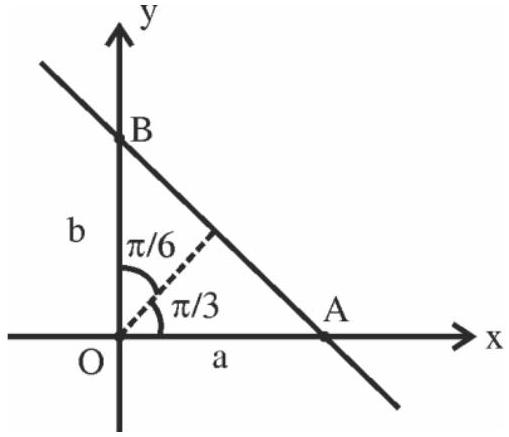
\includegraphics[max width=\textwidth, center]{2025_10_03_96e86532e9cc1b08fca5g-06}

Equation of straight line : \(\frac{\mathrm{x}}{\mathrm{a}}+\frac{\mathrm{y}}{\mathrm{b}}=1\)

Or \(x \cos \frac{\pi}{3}+y \sin \frac{\pi}{3}=p\)\\
\(\frac{x}{2}+\frac{y \sqrt{3}}{2}=p\)\\
\(\frac{\mathrm{x}}{3 \mathrm{p}}+\frac{\mathrm{y}}{2 \mathrm{p}}=1\)

Comparing both : \(\mathrm{a}=2 \mathrm{p}, \mathrm{b}=\frac{2 \mathrm{p}}{\sqrt{3}}\)\\
Now area of \(\Delta \mathrm{OAB}=\frac{1}{2} \cdot \mathrm{ab}=\frac{98}{3} \cdot \sqrt{3}\)\\
\(\frac{1}{2} \cdot 2 \mathrm{p} \cdot \frac{2 \mathrm{p}}{\sqrt{3}}=\frac{98}{3} \cdot \sqrt{3}\)\\
\(\mathrm{p}^{2}=49\)\\
\(\mathrm{a}^{2}-\mathrm{b}^{2}=4 \mathrm{p}^{2}-\frac{4 \mathrm{p}^{2}}{3}=\frac{2}{3} 4 \mathrm{p}^{2}\)\\
\(=\frac{8}{3} \cdot 49=\frac{392}{3}\)\\
77. The coefficient of \(x^{301}\) in \((1+x)^{500}+x(1+x)^{499}+x^{2}(1+x)^{498}+\ldots . .+x^{500}\) is:\\
(1) \({ }^{501} \mathrm{C}_{302}\)\\
(2) \({ }^{500} \mathrm{C}_{301}\)\\
(3) \({ }^{500} \mathrm{C}_{300}\)\\
(4) \({ }^{501} \mathrm{C}_{200}\)

Official Ans. by NTA (4)\\
Allen Ans. (4)\\
Sol. \((1+\mathrm{x})^{500}+\mathrm{x}(1+\mathrm{x})^{499}+\mathrm{x}^{2}(1+\mathrm{x})^{498}+\ldots .+\mathrm{x}^{500}\)

\[
\begin{aligned}
& =(1+\mathrm{x})^{500} \cdot\left\{\frac{1-\left(\frac{\mathrm{x}}{1+\mathrm{x}}\right)^{501}}{1-\frac{\mathrm{x}}{1+\mathrm{x}}}\right\} \\
& =(1+\mathrm{x})^{500} \frac{\left((1+\mathrm{x})^{501}-\mathrm{x}^{501}\right)}{(1+\mathrm{x})^{501}} \cdot(1+\mathrm{x}) \\
& =(1+\mathrm{x})^{501}-\mathrm{x}^{501}
\end{aligned}
\]

Coefficient of \(x^{301}\) in \((1+x)^{501}-x^{501}\) is given by \({ }^{501} \mathrm{C}_{301}={ }^{501} \mathrm{C}_{200}\)\\
78. Among the statements:\\
(S1) \(\quad((\mathrm{p} \vee \mathrm{q}) \Rightarrow \mathrm{r}) \Leftrightarrow(\mathrm{p} \Rightarrow \mathrm{r})\)\\
(S2) \(\quad((p \vee q) \Rightarrow r) \Leftrightarrow((p \Rightarrow r) \vee(q \Rightarrow r))\)\\
(1) Only (S1) is a tautology\\
(2) Neither (S1) nor (S2) is a tautology\\
(3) Only (S2) is a tautology\\
(4) Both (S1) and (S2) are tautologies

Official Ans. by NTA (2)\\
Allen Ans. (2)\\
Sol. \(\quad S_{1} \equiv((p \vee q) \Rightarrow r) \Leftrightarrow(p \Rightarrow r)\)

\begin{center}
\begin{tabular}{|l|l|l|l|l|l|l|}
\hline
p & q & r & \(\mathrm{p} \vee \mathrm{q}\) & \((\mathrm{p} \vee \mathrm{q}) \Rightarrow \mathrm{r}\) & \(\mathrm{p} \Rightarrow \mathrm{r}\) & \(((\mathrm{p} \vee \mathrm{q}) \Rightarrow \mathrm{r}) \Leftrightarrow(\mathrm{p} \Rightarrow \mathrm{r})\) \\
\hline
T & T & T & T & T & T & T \\
\hline
T & T & F & T & F & F & T \\
\hline
T & F & T & T & T & T & T \\
\hline
F & T & T & T & T & T & T \\
\hline
T & F & F & T & F & F & T \\
\hline
F & T & F & T & F & T & T \\
\hline
F & F & F & T & T & T & T \\
\hline
F & F & F & F & T & T & T \\
\hline
\end{tabular}
\end{center}

\begin{center}
\begin{tabular}{|l|l|l|l|l|l|l|l|}
\hline
\multicolumn{8}{|c|}{\(\mathrm{S}_{2} \equiv(\mathrm{p} \vee \mathrm{q}) \Rightarrow \mathrm{r} \Leftrightarrow((\mathrm{p} \Rightarrow \mathrm{r}) \vee(\mathrm{q} \Rightarrow \mathrm{r}))\)} \\
\hline
p & q & r & \((\mathrm{p} \vee \mathrm{q}) \Rightarrow \mathrm{r}\) & \(\mathrm{p} \Rightarrow \mathrm{r}\) & \(\mathrm{q} \Rightarrow \mathrm{r}\) & \((\mathrm{p} \Rightarrow \mathrm{r} \vee(\mathrm{q} \Rightarrow \mathrm{r}))\) & S2 \\
\hline
T & T & T & T & T & T & T & T \\
\hline
T & T & F & F & F & F & T & T \\
\hline
T & F & T & T & T & T & T & T \\
\hline
F & T & T & T & T & T & T & T \\
\hline
T & F & F & F & T & T & T & F \\
\hline
F & T & F & F & F & F & T & F \\
\hline
F & F & T & T & T & T & T & T \\
\hline
F & F & F & T & T & T & T & T \\
\hline
\end{tabular}
\end{center}

S2 \(\rightarrow\) not a tautology\\
79. The minimum number of elements that must be added to the relation \(\mathrm{R}=\{(\mathrm{a}, \mathrm{b}),(\mathrm{b}, \mathrm{c})\}\) on the set \(\{a, b, c\}\) so that it becomes symmetric and transitive is:\\
(1) 4\\
(2) 7\\
(3) 5\\
(4) 3

Official Ans. by NTA (2)\\
Allen Ans. (2)\\
Sol. For Symmetric \((a, b),(b, c) \in R\)\\
\(\Rightarrow(b, a),(c, b) \in R\)\\
For Transitive \((a, b),(b, c) \in R\)\\
\(\Rightarrow(a, c) \in R\)\\
Now

\begin{enumerate}
  \item Symmetric\\
\(\therefore(a, c) \in R \Rightarrow(c, a) \in R\)
  \item Transitive\\
\(\therefore(a, b),(b, a) \in R\)\\
\(\Rightarrow(a, a) \in R \&(b, c),(c, b) \in R\)\\
\(\Rightarrow(b, b) \&(c, c) \in R\)\\
\(\therefore\) Elements to be added\\
\(\left\{\begin{array}{r}(b, a),(c, b),(a, c),(c, a) \\ ,(a, a),(b, b),(c, c)\end{array}\right\}\)
\end{enumerate}

Number of elements to be added \(=7\)\\
80. If the solution of the equation \(\log _{\cos x} \cot x+4 \log _{\sin x} \tan x=1, x \in\left(0, \frac{\pi}{2}\right)\), is \(\sin ^{-1}\left(\frac{\alpha+\sqrt{\beta}}{2}\right)\), where \(\alpha, \beta\) are integers, then \(\alpha+\beta\) is equal to:\\
(1) 3\\
(2) 5\\
(3) 6\\
(4) 4

Official Ans. by NTA (4)\\
Allen Ans. (4)\\
Sol.\\
\(\log _{\cos x} \cot x+4 \log _{\sin x} \tan x=1\)\\
\(\Rightarrow \frac{\ln \cos x-\ln \sin x}{\ln \cos x}+4 \frac{\ln \sin x-\ln \cos x}{\ln \sin x}=1\)\\
\(\Rightarrow(\ln \sin x)^{2}-4(\ln \sin x)(\ln \cos x)+4(\ln \cos x)^{2}=1\)\\
\(\Rightarrow \ln \sin x=2 \ln \cos x\)\\
\(\Rightarrow \sin ^{2} x+\sin x-1=0 \Rightarrow \sin x=\frac{-1+\sqrt{5}}{2}\)\\
\(\therefore \alpha+\beta=4\)\\
Correct option (4)

\section*{SECTION-B}
\begin{enumerate}
  \setcounter{enumi}{80}
  \item Let \(S=\{1,2,3,4,5,6\}\). Then the number of oneone functions \(\mathrm{f}: \mathrm{S} \rightarrow \mathrm{P}(\mathrm{S})\), where \(\mathrm{P}(\mathrm{S})\) denote the power set of \(S\), such that \(f(n) \subset f(m)\) where \(\mathrm{n}<\mathrm{m}\) is \(\_\_\_\_\) .\\
Official Ans. by NTA (3240)\\
Allen Ans. (3240)\\
Sol. Let \(\mathrm{S}=\{1,2,3,4,5,6\}\), then the number of one-one functions, \(f: S \rightarrow P(S)\), where \(P(S)\) denotes the power set of \(S\), such that \(f(n)<f(m)\) where \(n<m\) is\\
\(n(S)=6\)\\
\(P(S)=\left\{\begin{array}{c}\phi,\{1\}, \ldots\{6\},\{1,2\}, \ldots, \\ \{5,6\}, \ldots,\{1,2,3,4,5,6\}\end{array}\right\}\)
\end{enumerate}

\begin{itemize}
  \item 64 elements\\
case-1\\
\(f(6)=\) S i.e. 1 option,\\
\(\mathrm{f}(5)=\) any 5 element subset A of S i.e. 6 options,\\
\(f(4)=\) any 4 element subset \(B\) of A i.e. 5 options,\\
\(\mathrm{f}(3)=\) any 3 element subset C of B i.e. 4 options,\\
\(\mathrm{f}(2)=\) any 2 element subset D of C i.e. 3 options,\\
f (1) = any 1 element subset E of D or empty subset i.e. 3\\
options,\\
Total functions = 1080\\
Case - 2\\
\(f(6)=\) any 5 element subset \(A\) of \(S\) i.e. 6 options,\\
\(\mathrm{f}(5)=\) any 4 element subset B of A i.e. 5 options,\\
\(\mathrm{f}^{\prime}(4)=\) any 3 element subset C of B i.e. 4 options,\\
\(f(3)=\) any 2 element subset \(D\) of \(C\) i.e. 3 options,\\
\(\mathrm{f}^{\prime}(2)=\) any 1 element subset E of D i.e. 2 options,\\
f \((1)=\) empty subset i.e. 1 option\\
Total functions \(=720\)\\
Case - 3\\
\(f(6)=S\)\\
\(\mathrm{f}(5)=\) any 4 element subset A of' S i.e. 15 options,\\
\(\mathrm{f}(4)=\) any 3 element subset B of A i.e. 4 options,\\
\(\mathrm{f}(3)=\) any 2 element subset C of B i.e. 3 options,\\
\(\mathrm{f}(2)=\) any 1 element subset D of C i.e. 2 options,\\
\(\mathrm{f}(1)=\) empty subset i.e. 1 option\\
Total functions \(=360\)\\
Case - 4\\
\(\mathrm{f}(6)=\mathrm{S}\)\\
\(\mathrm{f}(5)=\) any 5 element subset A of S i.e. 6 options,\\
\(f(4)=\) any 3 element subset \(B\) of \(A\) i.e. 10 options,\\
\(\mathrm{f}(3)=\) any 2 element subset C of B i.e. 3 options,\\
\(f(2)=\) any 1 element subset \(D\) of \(C\) i.e. 2 options,\\
\(\mathrm{f}(1)=\) empty subset i.e. 1 option\\
Total functions \(=360\)\\
Case - 5\\
\(\mathrm{f}(6)=\mathrm{S}\)\\
\(\mathrm{f}(5)=\) any 5 element subset A of S i.e. 6 options,\\
\(f(4)=\) any 4 element subset \(B\) of \(A\) i.e. 5 options,\\
\(\mathrm{f}(3)=\) any 2 element subset C of B i.e. 6 options,\\
\(\mathrm{f}(2)=\) any 1 element subset D of C i.e. 2 options,\\
\(\mathrm{f}(1)=\) empty subset i.e. 1 option\\
Total functions \(=360\)\\
Case - 6\\
\(\mathrm{f}(6)=\mathrm{S}\)\\
\(\mathrm{f}(5)=\) any 5 element subset A of S i.e. 6 options,\\
\(f(4)=\) any 4 element subset \(B\) of \(A\) i.e. 5 options,\\
\(\mathrm{f}(3)=\) any 3 element subset C of B i.e. 4 options,\\
\(f(2)=\) any 1 element subset \(D\) of \(C\) i.e. 3 options,\\
\(\mathrm{f}(1)=\) empty subset i.e. 1 option\\
Total functions \(=360\)\\
\(\therefore\) Number of such functions \(=3240\)
\end{itemize}

\begin{enumerate}
  \setcounter{enumi}{81}
  \item Let \(\alpha\) be the area of the larger region bounded by the curve \(\mathrm{y}^{2}=8 \mathrm{x}\) and the lines \(\mathrm{y}=\mathrm{x}\) and \(\mathrm{x}=2\), which lies in the first quadrant. Then the value of \(3 \alpha\) is equal to \(\_\_\_\_\) .
\end{enumerate}

Official Ans. by NTA (22)\\
Allen Ans. (22)\\
Sol.\\
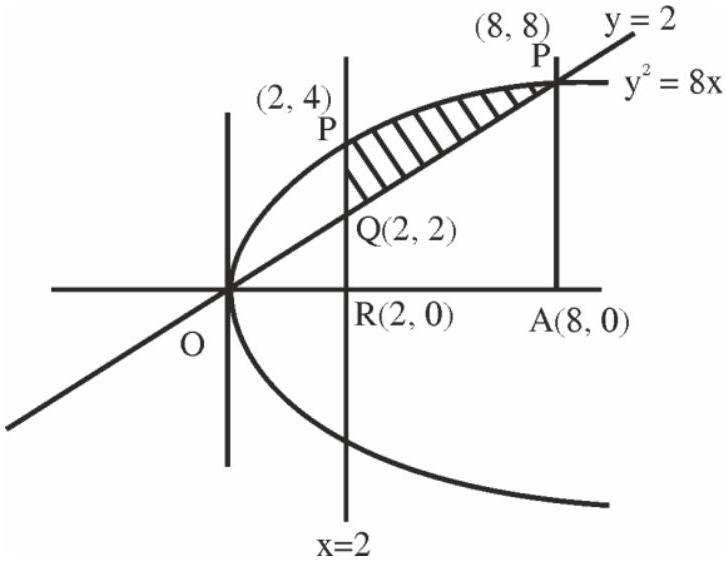
\includegraphics[max width=\textwidth, center]{2025_10_03_96e86532e9cc1b08fca5g-08}\\
\(y=x\)\\
\(\& \mathrm{y}^{2}=8 \mathrm{x}\)\\
Solving it

\[
\begin{array}{ll} 
& \mathrm{x}^{2}=8 \mathrm{x} \\
\therefore & \mathrm{x}=0,8 \\
\therefore & \mathrm{y}=0,8 \\
& \mathrm{x}=2 \text { will intersect occur at }
\end{array}
\]

\(y^{2}=16 \Rightarrow \quad y= \pm 4\)\\
\(\therefore \quad\) Area of shaded

\[
\begin{aligned}
& =\int_{2}^{8}(\sqrt{8 x}-x) d x=\int_{2}^{8}(2 \sqrt{2} \sqrt{x}-x) d x \\
& =\left[2 \sqrt{2} \cdot \frac{x^{3 / 2}}{3 / 2}-\frac{x^{2}}{2}\right]_{0}^{8} \\
& =\left(\frac{4 \sqrt{2}}{3} \cdot 2^{9 / 2}-32\right)-\left(\frac{4 \sqrt{2}}{3} \cdot 2^{9 / 2}-2\right) \\
& =\frac{128}{3}-32-\frac{16}{3}+2=\frac{112-90}{3}=\frac{22}{3}=\mathrm{A} \\
& \therefore 3 \mathrm{~A}=22
\end{aligned}
\]

\begin{enumerate}
  \setcounter{enumi}{82}
  \item If \(\lambda_{1}<\lambda_{2}\) are two values of \(\lambda\) such that the angle between the planes \(P_{1}: \vec{r}(3 \hat{i}-5 \hat{j}+k)=7\) and \(P_{2}: \vec{r} \cdot(\lambda \hat{i}+\hat{j}-3 k)=9\) is \(\sin ^{-1}\left(\frac{2 \sqrt{6}}{5}\right)\), then the square of the length of perpendicular from the point \(\left(38 \lambda_{1}, 10 \lambda_{2}, 2\right)\) to the plane \(\mathrm{P}_{1}\) is \(\_\_\_\_\) .
\end{enumerate}

\section*{Official Ans. by NTA (315)}
\section*{Allen Ans. (315)}
Sol. \(\quad P_{1}=\vec{r} \cdot(3 \hat{i}-5 \hat{j}+k)=7\)\\
\(P_{2}=\vec{r} \cdot(\lambda \hat{i}+\hat{j}-3 k)=9\)\\
\(\theta=\sin ^{-1}\left(\frac{2 \sqrt{6}}{5}\right)\)\\
\(\Rightarrow \sin \theta=\frac{2 \sqrt{6}}{5}\)\\
\(\therefore \cos \theta=\frac{1}{5}\).\\
\(\cos \theta=\frac{\overrightarrow{\mathrm{r}} \cdot \overrightarrow{\mathrm{r}}}{|\overrightarrow{\mathrm{r}} 1||\overrightarrow{\mathrm{r}} 2|}\)\\
\(=\frac{(3 \mathrm{i}-5 \mathrm{j}+\mathrm{K})(\lambda \mathrm{i}+\mathrm{j}-3 \mathrm{~K})}{\sqrt{35} \cdot \sqrt{\lambda^{2}+10}}\)\\
\(\frac{1}{5}=\left|\frac{3 \lambda-8}{\sqrt{35} \cdot \sqrt{\lambda^{2}+10}}\right|\)

Square \(\Rightarrow \frac{1}{25}=\frac{9 \lambda^{2}+64-48 \lambda}{35\left(\lambda^{2}+10\right)}\)\\
\(\Rightarrow 19 \lambda^{2}-120 \lambda+125=0\)\\
\(\Rightarrow 19 \lambda^{2}-95 \lambda-25 \lambda+125=0\)\\
\(\Rightarrow \mathrm{x}=5, \frac{25}{19}\)

Perpendicular distance of point\\
\(\left(38 \lambda_{1}, 10 \lambda_{2}, 2\right) \equiv(50,50,2)\) from plane \(\mathrm{P}_{1}\)\\
\(=\frac{|3 \times 50-5 \times 50+2-7|}{\sqrt{35}}=\frac{105}{\sqrt{35}}\)

Square \(=\frac{105 \times 105}{35}=315\)\\
84. Let \(z=1+i\) and \(z_{1}=\frac{1+i \bar{z}}{\bar{z}(1-z)+\frac{1}{z}}\). Then \(\frac{12}{\pi} \arg \left(z_{1}\right)\) is equal to \(\_\_\_\_\) .

Official Ans. by NTA (9)\\
Allen Ans. (9)\\
Sol. \(z=1+i\)

\[
\begin{aligned}
& z_{1}=\frac{1+i \bar{z}}{\bar{z}(1-z)+\frac{1}{z}} \\
& z_{1}=\frac{1+i(1-i)}{(1-i)(1-1-i)+\frac{1}{1+i}} \\
& =\frac{1+i-i^{2}}{(1-i)(-i)+\frac{1-i}{2}} \\
& =\frac{2+i}{\frac{-3 i-1}{2}}=\frac{4+2 i}{-3 i-1} \\
& =\frac{-(4+2 i)(3 i-1)}{(3 i)^{2}-(1)^{2}} \\
& \operatorname{Arg}\left(z_{1}\right)=\frac{3 \pi}{4} \\
& \therefore \frac{12}{\pi} \arg \left(z_{1}\right)=\frac{12}{\pi} \times \frac{3 \pi}{4}=9
\end{aligned}
\]

\begin{enumerate}
  \setcounter{enumi}{84}
  \item \(\lim _{x \rightarrow 0} \frac{48}{x^{4}} \int_{0}^{x} \frac{t^{3}}{t^{6}+1} d t\) is equal to \(\_\_\_\_\) .\\
Official Ans. by NTA (12)\\
Allen Ans. (12)\\
Sol. \(\quad 48 \lim _{x \rightarrow 0} \frac{\int_{0}^{x} \frac{t^{3}}{t^{6}+1} d t}{x^{4}}\left(\frac{0}{0}\right)\)\\
Applying L' Hospitals Rule\\
\(48 \lim _{x \rightarrow 0} \frac{x^{3}}{x^{6}+1} \times \frac{1}{4 x^{3}}\)\\
\(=12\)
  \item The mean and variance of 7 observations are 8 and 16 respectively. If one observation 14 is omitted a and \(b\) are respectively mean and variance of remaining 6 observation, then \(\mathrm{a}+3 \mathrm{~b}-5\) is equal to \(\_\_\_\_\) .\\
Official Ans. by NTA (37)\\
Allen Ans. (37)\\
Sol. \(\frac{x_{1}+x_{2}+\ldots .+x_{7}}{7}=8\)\\
\(\frac{x_{1}+x_{2}+x_{3} \ldots .+x_{6}+14}{7}=8\)\\
\(\Rightarrow \mathrm{x}_{1}+\mathrm{x}_{2}+\ldots .+\mathrm{x}_{6}=42\)\\
\(\therefore \frac{\mathrm{x}_{1}+\mathrm{x}_{2} \ldots .+\mathrm{x}_{6}}{6}=\frac{42}{6}=7=\mathrm{a}\)\\
\(\frac{\Sigma \mathrm{x}_{\mathrm{i}}{ }^{2}}{7}-8^{2}=16\)\\
\(\Sigma x i^{2}=560\)\\
\(\Rightarrow \mathrm{x}_{1}^{2}+\mathrm{x}_{2}^{2}+\ldots+\mathrm{x}_{6}^{2}=364\)\\
\(\mathrm{b}=\frac{\mathrm{x}_{1}^{2}+\mathrm{x}_{2}^{2}+\ldots .+\mathrm{x}_{6}^{2}}{6}-7^{2}\)\\
\(=\frac{364}{6}-49\)\\
\(\mathrm{b}=\frac{70}{6}\)\\
\(a+3 b-5=7+3 \times \frac{70}{6}-5\)\\
\(=37\)
  \item If the equation of the plane passing through the point \((1,1,2)\) and perpendicular to the line \(\mathrm{x}-3 \mathrm{y}+2 \mathrm{z}-1=04 \mathrm{x}-\mathrm{y}+\mathrm{z}\) is \(\mathrm{Ax}+\mathrm{By}+\mathrm{Cz}=1\), then \(140(C-B+A)\) is equal to \(\_\_\_\_\) .
\end{enumerate}

Official Ans. by NTA (15)\\
Allen Ans. (15)\\
Sol. \(\quad x-3 y+2 z-1=0\)\\
\(4 x-y+z=0\)\\
\(\overrightarrow{\mathrm{n}}_{1} \times \overrightarrow{\mathrm{n}}_{2}=\left|\begin{array}{ccc}\hat{\mathrm{i}} & \hat{\mathrm{j}} & \mathrm{k} \\ 1 & -3 & 2 \\ 4 & -1 & 1\end{array}\right|\)\\
\(=-\hat{\mathrm{i}}+7 \hat{\mathrm{j}}+11 \mathrm{k}\)

Dr \(^{\mathrm{s}}\) of normal to the plane is \(-1,7,11\)

Equation of plane :\\
\(-1(x-1)+7(y-1)+11(z-2)=0\)\\
\(-x+7 y+11 z=28\)\\
\(\frac{-1}{28} x+\frac{7 y}{28}+\frac{11 z}{28}=1\)\\
\(\mathrm{Ax}+\mathrm{By}+\mathrm{Cz}=1\)\\
\(140(\mathrm{C}-\mathrm{B}+\mathrm{A})=140\left(\frac{11}{28}-\frac{7}{28}-\frac{1}{28}\right)\)\\
\(=140 \times \frac{3}{28}=15\)\\
88. Let \(\sum_{n=0}^{\infty} \frac{n^{3}((2 n)!)+(2 n-1)(n!)}{(n!)((2 n)!)}=a e+\frac{b}{e}+c\),\\
where \(a, b, c \in \mathbb{Z}\) and \(e=\sum_{n=0}^{\infty} \frac{1}{n!}\) Then \(a^{2}-b+c\) is equal to \(\_\_\_\_\) .\\
Official Ans. by NTA (26)\\
Allen Ans. (26)

Sol. \(\quad \sum_{n=0}^{\infty} \frac{n^{3}((2 n)!)+(2 n-1)(n!)}{(n!)((2 n)!)}\)\\
\(=\sum_{n=0}^{\infty} \frac{1}{(n-3)!}+\sum_{n=0}^{\infty} \frac{3}{(n-2)!}\)\\
\(+\sum_{n=0}^{\infty} \frac{1}{(n-1)!}+\sum_{n=0}^{\infty} \frac{1}{(2 n-1)!}-\sum_{n=0}^{\infty} \frac{1}{(2 n)!}\)\\
\(=e+3 e+e+\frac{1}{2}\left(e-\frac{1}{e}\right)-\frac{1}{2}\left(e+\frac{1}{e}\right)\)\\
\(=5 e-\frac{1}{e}\)\\
\(\therefore a^{2}-b+c=26\)\\
89. Number of 4-digit numbers (the repetition of digits is allowed) which are made using the digits \(1,2,3\) and 5 , and are divisible by 15 , is equal to \(\_\_\_\_\)\\
Official Ans. by NTA (21)\\
Allen Ans. (21)\\
Sol. For number to be divisible by 15 , last digit should be 5 and sum of digits must be divisible by 3 .

Possible combinations are

\begin{center}
\begin{tabular}{|l|l|l|l|}
\hline
1 & 2 & 1 & 5 \\
\hline
\end{tabular}
\end{center}

Numbers \(=3\)

\begin{center}
\begin{tabular}{|l|l|l|l|}
\hline
2 & 2 & 3 & 5 \\
\hline
\end{tabular}
\end{center}

Numbers \(=3\)

\begin{center}
\begin{tabular}{|l|l|l|l|}
\hline
3 & 3 & 1 & 5 \\
\hline
\end{tabular}
\end{center}

Numbers \(=3\)

\begin{center}
\begin{tabular}{|l|l|l|l|}
\hline
1 & 1 & 5 & 5 \\
\hline
\end{tabular}
\end{center}

Numbers \(=3\)

\begin{center}
\begin{tabular}{|l|l|l|l|}
\hline
2 & 3 & 5 & 5 \\
\hline
\end{tabular}
\end{center}

Numbers \(=6\)

\begin{center}
\begin{tabular}{|l|l|l|l|}
\hline
3 & 5 & 5 & 5 \\
\hline
\end{tabular}
\end{center}

Numbers \(=3\)

Total Numbers \(=21\)\\
90. Let \(f^{1}(x)=\frac{3 x+2}{2 x+3}, x \in R-\left\{\frac{-3}{2}\right\}\)

For \(\mathrm{n} \geq 2\), define \(\mathrm{f}^{\mathrm{n}}(\mathrm{x})=\mathrm{f}^{1} 0 \mathrm{f}^{\mathrm{n}-1}(\mathrm{x})\).\\
If \(\mathrm{f}^{5}(\mathrm{x})=\frac{\mathrm{ax}+\mathrm{b}}{\mathrm{bx}+\mathrm{a}}, \operatorname{gcd}(\mathrm{a}, \mathrm{b})=1\), then \(\mathrm{a}+\mathrm{b}\) is equal to \(\_\_\_\_\) .

Official Ans. by NTA (3125)\\
Allen Ans. (3125 )

Sol.

\[
\begin{aligned}
& f^{1}(x)=\frac{3 x+2}{2 x+3} \\
& \Rightarrow f^{2}(x)=\frac{13 x+12}{12 x+13} \\
& \Rightarrow f^{3}(x)=\frac{63 x+62}{62 x+63} \\
& \therefore f^{5}(x)=\frac{1563 x+1562}{1562 x+1563} \\
& a+b=3125
\end{aligned}
\]


\end{document}